\section{From Voxel Representation to Parametrized Surface Points}
\label{sec:surfaceImpl}
Surface extraction is an intermediate step between topology optimization and \ac{NURBS} representation. This intermediate step is crucial, because it generates the data for the \ac{NURBS} surface fitting and for the underlying topology of the \ac{NURBS} patches.

%Subsection on surface reconstruction
\subsection{Surface reconstruction}
In \autoref{sec:surfaceBackg} different surface reconstruction schemes have been introduced. In the following we want to discuss our choice for an appropriate surface reconstruction scheme and explain necessary modifications to it.

\subsubsection{Discussion on surface reconstruction schemes}
\tododone[inline]{proofreading Benni\& JC}
Since the surface reconstruction is just an intermediate step before our final \ac{NURBS} fitting procedure, it is not sufficient to only produce a good surface approximation of our optimized topology, but additional constraints have to be kept in mind:
\begin{enumerate}
\item \ac{NURBS} have a rectangular topology, therefore our surface reconstruction should also be able to provide a surface consisting of rectangular patches.
\item Peters' Scheme only covers manifold surfaces, meaning that per edge each patch is only allowed to have exactly one neighbour.
\end{enumerate}
The first requirement is met by \ac{DC}, while the second one is only met by \ac{MC}. We decided to use the \ac{DC} method, because already the basic version of it creates \acp{quad}, while \ac{MC} creates a mesh of triangles, which can only be changed into a mesh of \acp{quad} by considerably increasing the number of faces.

\subsubsection{Our implementation of \ac{DC}}
\tododone[inline]{proofreading Benni\& JC}
We used the open-source language PYTHON \cite{Python} for the implementation of \ac{DC}. Compared to the version described in \cite{Hermite2002} we applied some simplifications:
\begin{itemize}
\item We do not care about sharp features and cannot easily access gradient information in our algorithm. Therefore, we did not use \autoref{eq:QEF} for the generation of new vertices, but the simple averaging scheme described in \autoref{ssec:DC}.
\item For the reason that our dataset only consists of boolean values instead of real valued quantities, we locate our surface at the interface of material and no-material and not at a certain isovalue.
\item We did not implement the adaptive and topology safe scheme but a scheme for uniform grids which does not support adaptive mesh simplification nor topology checks.
\end{itemize}
This leads to the following modified \ac{DC} scheme:
\begin{enumerate}
\item On each cube edge find the root (i.e. the interface of material and no-material voxels) using bisection. We assume our surface to exactly lie in the middle between material and no-material voxels.
\item Take the mean value of all root positions for determining the position of the newly introduced vertex.
\item Join the vertices associated with four cubes sharing a common edge to form a \ac{quad}.
\end{enumerate}
So far our procedure generates \ac{quad} surfaces for boolean datasets on uniform Cartesian grids. But like for the original \ac{DC} algorithm we cannot guarantee that those surfaces are manifold.

\subsubsection{Obtaining manifold surfaces}
%\todointernal[inline]{proofreading!}
Since we want to deduce a first estimate for the topology of the \ac{NURBS} surface output of our \ac{CADTopOpt} tool, non-manifold surfaces cannot be accepted\footnote{Surfaces consisting of smoothly connected \ac{NURBS} \acp{patch} are always manifold surfaces. Therefore we cannot start with a non-manifold surface and assume we will end up with a manifold surface.}. We implemented a remeshing procedure for generating manifold surfaces out of non-manifold surfaces.

Our procedure has the following steps:
\begin{enumerate}
\item Find all non-manifold edges which are connected to more than two \acp{quad}.
\item All non-manifold edges are split into two manifold edges with only two \acp{quad} connected to them.
\item The members of each pair of manifold edges are moved into opposite directions. 
\end{enumerate}
The directions in which we are moving the resulting manifold edges can be determined by estimating the gradient at the position of the former non-manifold edge. Please note that we can only estimate the gradient if additional information in the middle of the faces penetrated by non-manifold edges is available. Otherwise it is not possible to resolve the ambiguity in a proper way and therefore we cannot eliminate the non-manifold edge. 
\todointern[inline]{add a picture for explanation!}
\tododone[inline]{I dont understand this sentence Benni}

We illustrate the procedure for a 2D example in \autoref{fig:manifoldResolution2D}. Please note that for the 3D case additional patterns occur and not only the \acp{quad} which are connected to the whole non-manifold edge have to be considered, but also the \acp{quad} connected to only one vertex of the edge. This also implies the introduction of new \acp{quad} at other locations (\autoref{fig:manifoldPatterns3D}).

\begin{figure}
\begin{center}
\begin{subfigure}[b]{.5\linewidth}
\centering
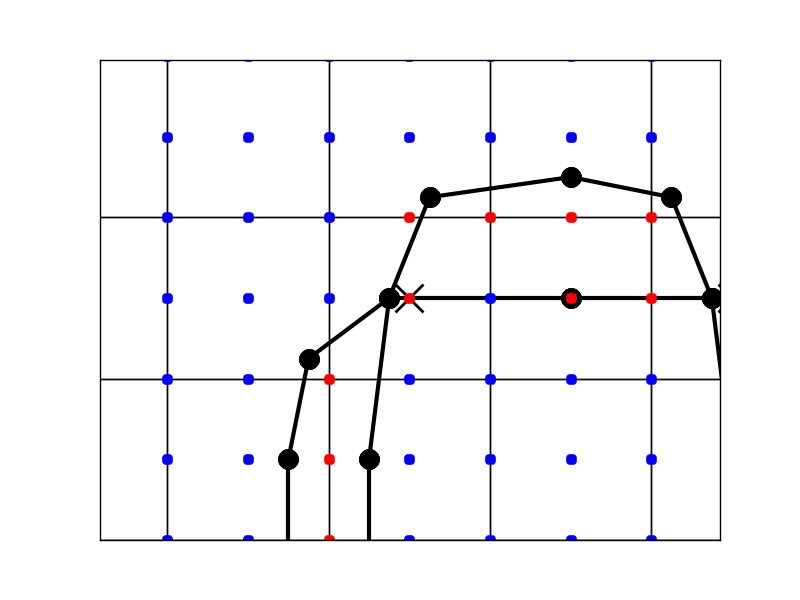
\includegraphics[width = \textwidth]{Pictures/SurfaceReconstruction/2DDoubleTorusNonManifoldDetail}
\subcaption{contour before remeshing}
\end{subfigure}%
\begin{subfigure}[b]{.5\linewidth}
\centering
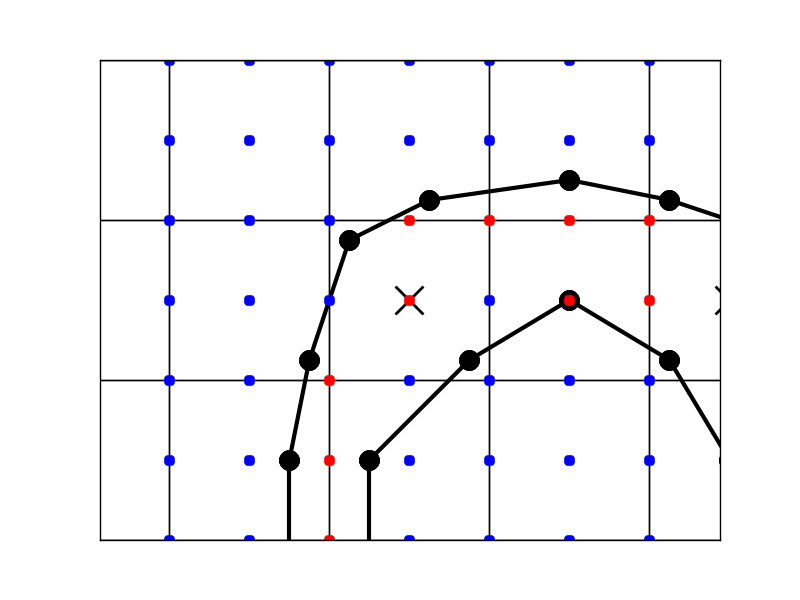
\includegraphics[width = \textwidth]{Pictures/SurfaceReconstruction/2DDoubleTorusManifoldDetail}
\subcaption{contour after remeshing}
\end{subfigure}
\end{center}
\caption{Illustration of the remeshing process. Blue dots denote outside voxels, red dots inside voxels, crosses denote voxels considered for resolving ambiguities}
\label{fig:manifoldResolution2D}
\end{figure}

\begin{figure}[p]
\begin{center}
\begin{subfigure}[b]{.45\textwidth}
\centering
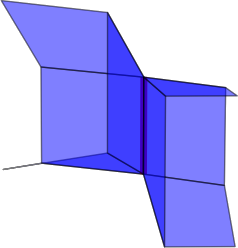
\includegraphics[height = .17\textheight, width = .5\textwidth,keepaspectratio]{Pictures/SurfaceReconstruction/3DManifoldOO}
\end{subfigure}
\begin{subfigure}[b]{.45\textwidth}
\centering
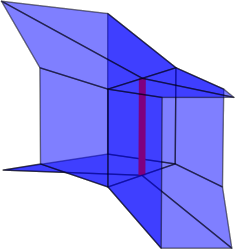
\includegraphics[height = .17\textheight, width = .5\textwidth,keepaspectratio]{Pictures/SurfaceReconstruction/3DManifoldOORes}
\end{subfigure}
\begin{subfigure}[b]{.45\textwidth}
\centering
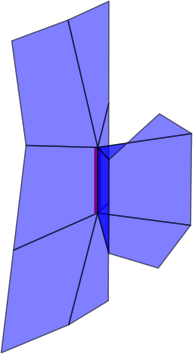
\includegraphics[height = .17\textheight, width = .5\textwidth,keepaspectratio]{Pictures/SurfaceReconstruction/3DManifoldII}
\end{subfigure}
\begin{subfigure}[b]{.45\textwidth}
\centering
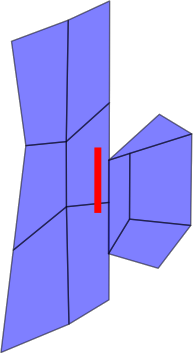
\includegraphics[height = .17\textheight, width = .5\textwidth,keepaspectratio]{Pictures/SurfaceReconstruction/3DManifoldIIRes}
\end{subfigure}
\begin{subfigure}[b]{.45\textwidth}
\centering
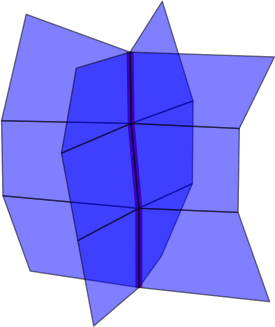
\includegraphics[height = .17\textheight, width = .5\textwidth,keepaspectratio]{Pictures/SurfaceReconstruction/3DManifoldMM}
\end{subfigure}
\begin{subfigure}[b]{.45\textwidth}
\centering
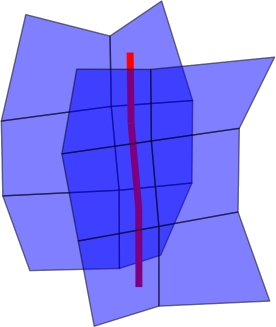
\includegraphics[height = .17\textheight, width = .5\textwidth,keepaspectratio]{Pictures/SurfaceReconstruction/3DManifoldMMRes}
\end{subfigure}
\begin{subfigure}[b]{.45\textwidth}
\centering
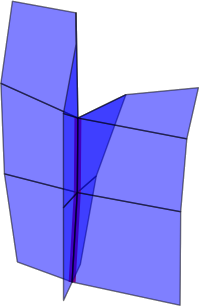
\includegraphics[height = .17\textheight, width = .5\textwidth,keepaspectratio]{Pictures/SurfaceReconstruction/3DManifoldMI}
\end{subfigure}
\begin{subfigure}[b]{.45\textwidth}
\centering
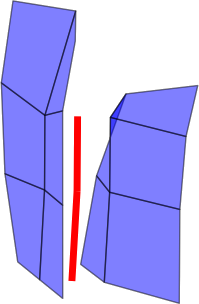
\includegraphics[height = .17\textheight, width = .5\textwidth,keepaspectratio]{Pictures/SurfaceReconstruction/3DManifoldMIRes}
\end{subfigure}
\begin{subfigure}[b]{.45\textwidth}
\centering
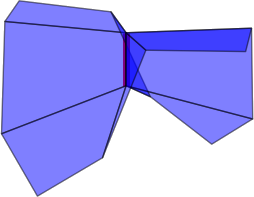
\includegraphics[height = .17\textheight, width = .5\textwidth,keepaspectratio]{Pictures/SurfaceReconstruction/3DManifoldOI}
\end{subfigure}
\begin{subfigure}[b]{.45\textwidth}
\centering
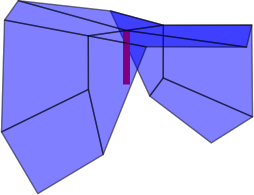
\includegraphics[height = .17\textheight, width = .5\textwidth,keepaspectratio]{Pictures/SurfaceReconstruction/3DManifoldOIRes}
\end{subfigure}
\end{center}
\caption{Different patterns before (left) and after (right) remeshing. Depending on the neighbourhood of the non-manifold edge different patterns are applied. A non-manifold edge is connected to outside-outside (1.row), inside-inside (2.row), two other manifold edges (3.row), inside and another manifold edge (4.row), inside-outside (5.row). Please note that this figure does not cover all possible patterns.}
\label{fig:manifoldPatterns3D}
\end{figure}







\begin{comment}
\begin{table}
\begin{center}
\begin{tabularx}{.7\textwidth}{|*3{>{\centering\arraybackslash}X}|}
\hline
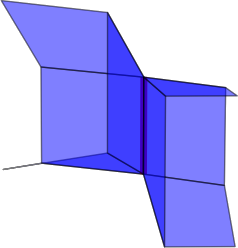
\includegraphics[height=.15\textheight]{Pictures/SurfaceReconstruction/3DManifoldOO}
&
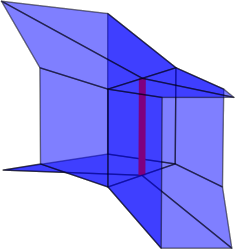
\includegraphics[height=.15\textheight]{Pictures/SurfaceReconstruction/3DManifoldOORes}
\\
\hline
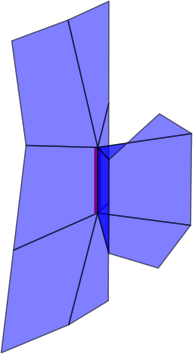
\includegraphics[height=.15\textheight]{Pictures/SurfaceReconstruction/3DManifoldII}
&
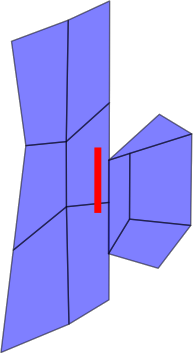
\includegraphics[height=.15\textheight]{Pictures/SurfaceReconstruction/3DManifoldIIRes}
\\
\hline
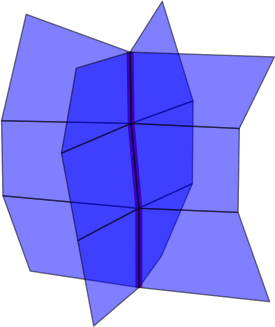
\includegraphics[height=.15\textheight]{Pictures/SurfaceReconstruction/3DManifoldMM}
&
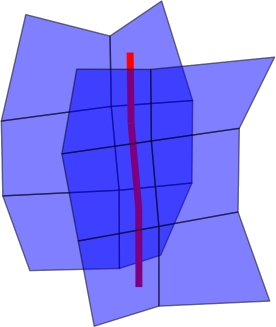
\includegraphics[height=.15\textheight]{Pictures/SurfaceReconstruction/3DManifoldMMRes}
\\
\hline
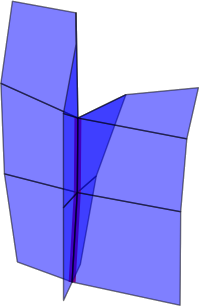
\includegraphics[height=.15\textheight]{Pictures/SurfaceReconstruction/3DManifoldMI}
&
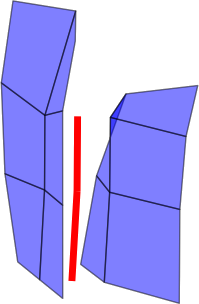
\includegraphics[height=.15\textheight]{Pictures/SurfaceReconstruction/3DManifoldMIRes}
\\
\hline
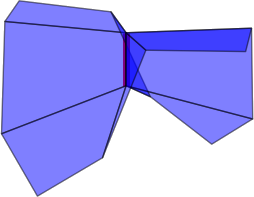
\includegraphics[height=.15\textheight]{Pictures/SurfaceReconstruction/3DManifoldOI}
&
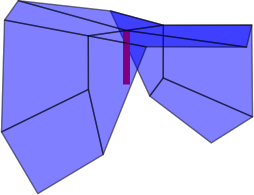
\includegraphics[height=.15\textheight]{Pictures/SurfaceReconstruction/3DManifoldOIRes}
\\
\hline
\end{tabularx}
\end{center}
\end{table}
\end{comment}

\begin{comment}
\begin{figure}[p]
\begin{minipage}[b][.17\textheight]{.45\textwidth}
\begin{center}
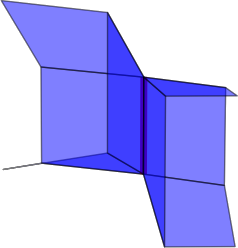
\includegraphics[height=.15\textheight]{Pictures/SurfaceReconstruction/3DManifoldOO}
\end{center}
\end{minipage}
\begin{minipage}[b][.17\textheight]{.45\textwidth}
\begin{center}
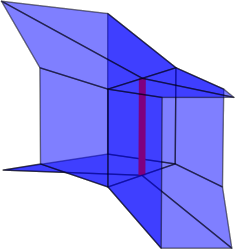
\includegraphics[height=.15\textheight]{Pictures/SurfaceReconstruction/3DManifoldOORes}
\end{center}
\end{minipage}
\begin{minipage}[b][.17\textheight]{.45\textwidth}
\begin{center}
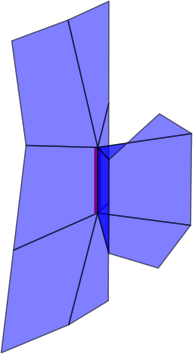
\includegraphics[height=.15\textheight]{Pictures/SurfaceReconstruction/3DManifoldII}
\end{center}
\end{minipage}
\begin{minipage}[b][.17\textheight]{.45\textwidth}
\begin{center}
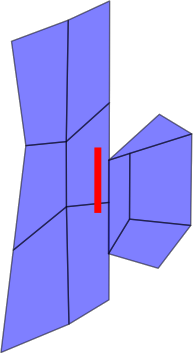
\includegraphics[height=.15\textheight]{Pictures/SurfaceReconstruction/3DManifoldIIRes}
\end{center}
\end{minipage}
\begin{minipage}[b][.17\textheight]{.45\textwidth}
\begin{center}
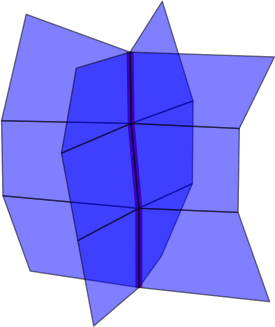
\includegraphics[height=.15\textheight]{Pictures/SurfaceReconstruction/3DManifoldMM}
\end{center}
\end{minipage}
\begin{minipage}[b][.17\textheight]{.45\textwidth}
\begin{center}
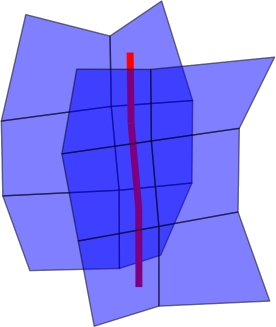
\includegraphics[height=.15\textheight]{Pictures/SurfaceReconstruction/3DManifoldMMRes}
\end{center}
\end{minipage}
\begin{minipage}[b][.17\textheight]{.45\textwidth}
\begin{center}
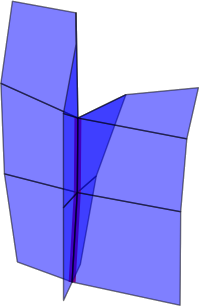
\includegraphics[height=.15\textheight]{Pictures/SurfaceReconstruction/3DManifoldMI}
\end{center}
\end{minipage}
\begin{minipage}[b][.17\textheight]{.45\textwidth}
\begin{center}
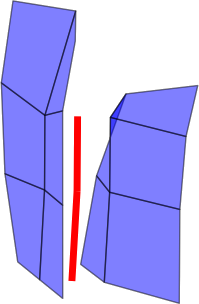
\includegraphics[height=.15\textheight]{Pictures/SurfaceReconstruction/3DManifoldMIRes}
\end{center}
\end{minipage}
\begin{minipage}[b][.17\textheight]{.45\textwidth}
\begin{center}
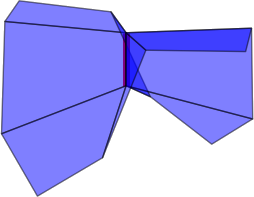
\includegraphics[height=.15\textheight]{Pictures/SurfaceReconstruction/3DManifoldOI}
\end{center}
\end{minipage}
\begin{minipage}[b][.17\textheight]{.45\textwidth}
\begin{center}
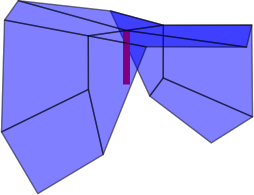
\includegraphics[height=.15\textheight]{Pictures/SurfaceReconstruction/3DManifoldOIRes}
\end{center}
\end{minipage}
\caption{Remeshing schemes for different kinds of manifold edges}
\label{fig:manifoldPatterns3D}
\end{figure}
\end{comment}

\begin{comment}

\subsubsection{Topology--safe adaptivity \ac{DC}}
\todo[inline]{Benni: this is a outlook, remove, put into comment.}
Implementing this feature in \ac{DC} will be one of our major goals in the future. Whether adding adaptivity to the basic \ac{DC} algorithm will destroy the property of \ac{DC} only generating \acp{quad} by introducing \acp{tri}, is going to be part of our future research.

\end{comment}

%Subsection on parametrization
\subsection{Parametrization of Datapoints}
\label{ssec:parametrization}
In addition to the reconstructed surface we need the following information for the least squares fit: 
\begin{itemize}
\item Which \ac{NURBS}-patch does each datapoint of the reconstructed surface belong to?
\item What are the values of $u,v$ parameters of the datapoint on the patch?
\end{itemize}
\subsubsection{Two-scale Dual Contouring}
Before we can distribute datapoints to \ac{NURBS}-patches, we first have to find out how these patches look like. Since we want to have as few patches as possible we do not simply turn every \ac{quad} from the surface reconstruction into a patch. Instead  we try to find a surface with as few \acp{quad} as possible, while keeping the same topology as our initially reconstructed surface. This coarse surface will be assumed to be the patch distribution for the later steps.


Therefore, in our algorithm we are reconstructing the surface on two different scales: a coarse and a fine scale. The coarse scale data is deduced from the fine scale data by recursively applying the following algorithm:
\begin{enumerate}
\item Combine sets of eight connected voxels with egde-length $a$ into a coarse voxel with edgelength $2a$ (see \autoref{sfig:coarsenA}).
\item Decide whether the new voxel resembles an inner ($=1$) or outer ($=0$) voxel. This is done by taking the mean value of the contributing eight voxels. If the mean value is above a certain threshold $t$, the new voxel is considered as an inner voxel. We picked $t=\frac{1}{8}$, i.e. if at least two voxels out of eight are inner voxels, the resulting voxel is considered being an inner voxel.
\item For the resolution of non-manifold edges, additional coarse voxel grids are generated. These grids are shifted by edge-length $a$ (see \autoref{sfig:coarsenB}).
\end{enumerate}
\begin{figure}
\begin{subfigure}{.45\textwidth}
\begin{center}
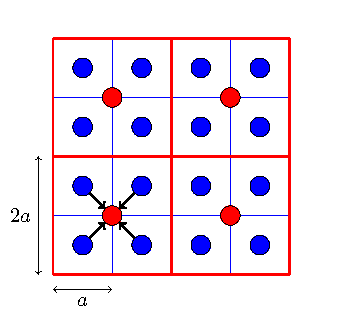
\includegraphics[scale=1]{Pictures/tikzCoarsen/coarsen.pdf}
\end{center}
\subcaption{Sets of 8 (4 in 2D) fine voxels (blue) are recursively combined to form one coarse voxel (red).}
\label{sfig:coarsenA}
\end{subfigure}\hfill
\begin{subfigure}{.45\textwidth}
\begin{center}
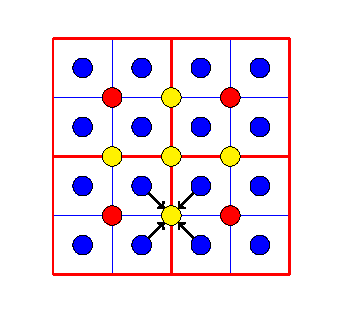
\includegraphics[scale=1]{Pictures/tikzCoarsen/coarsenMani.pdf}
\end{center}
\subcaption{Addition voxels (yellow) are introduced in a non-aligned grid for non-manifold resolution on the coarse scale.}
\label{sfig:coarsenB}
\end{subfigure}
\caption{Coarsening scheme applied in \emph{Two-scale \acl{DC}}.}
\label{fig:coarsen}
\end{figure}
One iteration of this coarsening scheme is referred to as one \emph{coarsening step}. Applying this scheme recursively allows higher coarsening and results in multiple coarsening steps.

Here, we apply \ac{DC} to both datasets and obtain two different reconstructed surfaces.
The coarse scale surface is used as a patch distribution and from the fine scale we obtain our datapoints. The \ac{NURBS} will be fitted to these datapoints. We call this approach \emph{Two-scale \acl{DC}} (see \autoref{fig:TwoScale}).
Of course this simple approach comes with drawbacks:
\begin{itemize}
\item We cannot guarantee that the coarse and the fine scale have exactly the same topology. Topological details of the fine scale, which do not exist on the coarse scale, are lost.
\item Both resolutions have to be chosen manually, since we do not have a criterion for evaluating the quality of the coarse scale surface reconstruction.
\end{itemize}
These drawbacks are especially bad for complex surfaces -- like the output of topology optimization -- where the topological details mentioned above are not an exception, but the default case. There are more elaborate surface extraction schemes that handle these problems. For the interested reader, alternative schemes such as \emph{Dual Marching Cubes} \cite{ScottSchaefer2004} or \emph{Manifold Dual Contouring} \cite{Schaefer2007}, are included in \autoref{appx:AltSurfRecon}.
\subsubsection{Projection of Datapoints onto Quads}
\label{sssec:projection}
Now that we have constructed a \ac{NURBS}-patch distribution, we can estimate the parametrization of the datapoints on the fine scale by projecting them onto the patches: 

For this procedure we do the following steps:

\begin{enumerate}
\item Find out onto which of these patches a datapoint should be projected. This can be done by simply measuring the distance from the datapoint to the centroid of each patch and deciding to project onto the patch with the smallest distance.
\item Project the point onto the target patch. For this, we want the whole \ac{quad} to be parametrized on $\left(u,v\right)\in\left[0,1\right]^2$. This is done by first approximating the quad (which may not necessarily be planar) with its least squares fit plane. Then a projection onto this plane is done by applying a simple basis transformation\footnote{This basis transformation is computed in a very efficient way by computing the QR-decomposition for the basis of each patch only once and applying it to each datapoint projected onto this patch.}.
\end{enumerate}

The projection might lead to parameters $\left(u,v\right)\not\in\left[0,1\right]^2$ for some of the datapoints. As we only produce surfaces for $\left(u,v\right)\in\left[0,1\right]^2$, these are then not on the surface. If we still include them in the fitting, these will then influence parts of the surface that are not there, leading to unwanted fitting behaviour such as wiggles and turns. 

We have tried several methods to solve this problem. For example, one might consider scaling the parameter space of each quad to $\left[0,1\right]^2$, which however leads to inconsistencies in parameter assignemt between neighbouring quads with different scaling. Another solution, cropping the parameter domain by shifting all parameters outside $\left[0,1\right]^2$ to the closest border (i.e. for $u \text{ or } v < 0$ is assigned to $0$, $u \text{ or } v >1$ is assigned to $1$), also leads to problems, as points in different regions of space then can end up having the same parameter values. To simplify the treatment, we therefore currently only consider the points parametrized inside $\left[0,1\right]^2$, and omit all points outside from this step onwards.

After completing all these steps we obtain the following data for the subsequent steps of our algorithm:
\begin{itemize}
\item a coarse surface delivering the topology for our \ac{NURBS}-patches in Peters' Scheme
\item a set of datapoints from the fine scale with coordinates $\left(x,y,z\right)^T\in\mathbb{R}^3$ and parameters $\left(u,v\right)\in\left[0,1\right]^2$, where each datapoint is associated with a \ac{NURBS}-patch. 
\end{itemize}
For a sample output of our algorithm for a 2D case, see \autoref{fig:TwoScale}.

\begin{figure}
\begin{center}
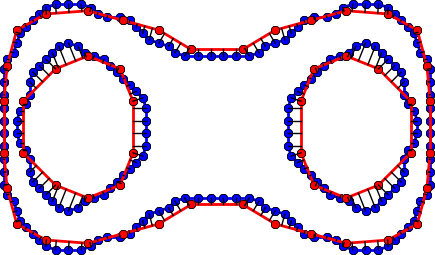
\includegraphics[width=.5 \textwidth]{Pictures/SurfaceReconstruction/TwoScale}
\caption{Twoscale \acl{DC} with a coarse surface reconstruction (red) and a fine one (blue). The datapoints from the fine scale are projected onto the edges from the coarse scale (black lines).}
\label{fig:TwoScale}
\end{center}
\end{figure}
\newpage
\begin{comment}
\subsubsection{Parameter estimation}
\todo[inline]{explain different strategies, comparison of final results would be great (could also be part of third milestone?)}
\todo[inline]{show possible problems}
\end{comment}


\begin{comment}
%In terms of implementing the surface extraction, we used VTK \cite{VTKToolbox}\todo{this has changed!}.

%\subsection{VTK Toolbox}


%The VTK toolbox was used in order to implement the algorithms on our optimized data. It is a heavily object
%oriented toolbox. Our first approach was to use the built in Marching Cubes algorithm,
%nevertheless it did not work with our unstructured grid data. It just works for ImageData and
%PolyData . For structured and unstructured grids the tool to render the isosurface is the \textit{Contour Filter} tool. Unfortunately the documentation does not present which algorithm the tool uses. It
%can be inferred that it is an extended Marching cubes algorithm.

The VTK Toolbox is an open-source tool, providing algorithms for "3D computer graphics, image processing, and visualization" \cite{VTKToolbox}. Among the variety of tools, VTK offers algorithms that allow us to obtain a surface representation from voxel data. Among these algorithms, we could find Marching Cubes, Dual Contouring and also a Decimation tool, the last of which can useful for reducing the data size further for the NURBS-representation step.


%\subsection{Implementation}
The Marching Cubes implementation in VTK is however not applicable to the VTK \emph{Unstructured Grid} type data that we obtain from ToPy, since it only works with \emph{Image Data} and \emph{PolyData}, the main data types in VTK. For structured and unstructured grids the tool to render the isosurface is the \emph{Contour Filter} tool. Unfortunately, the documentation does not present which algorithm the tool uses. It can be inferred that it is an extended Marching Cubes algorithm. %how?
Although an implementation with Contour Filtering worked, the visualization of the data was still not possible
making an intermediate step needed. Here, we used the \textit{Implicit Modelling} tool, a filter that
computes the distance from the input geometry to the points of an output structured point set.
This distance function can then be "contoured" to generate new, offset surfaces from the original
geometry. Although this approach allowed the visualisation, some crucial information was lost, as for example holes were not represented in the final model. This can be seen in \autoref{fig:contouring}.


\begin{figure}
\centering
   \scalebox{0.4}{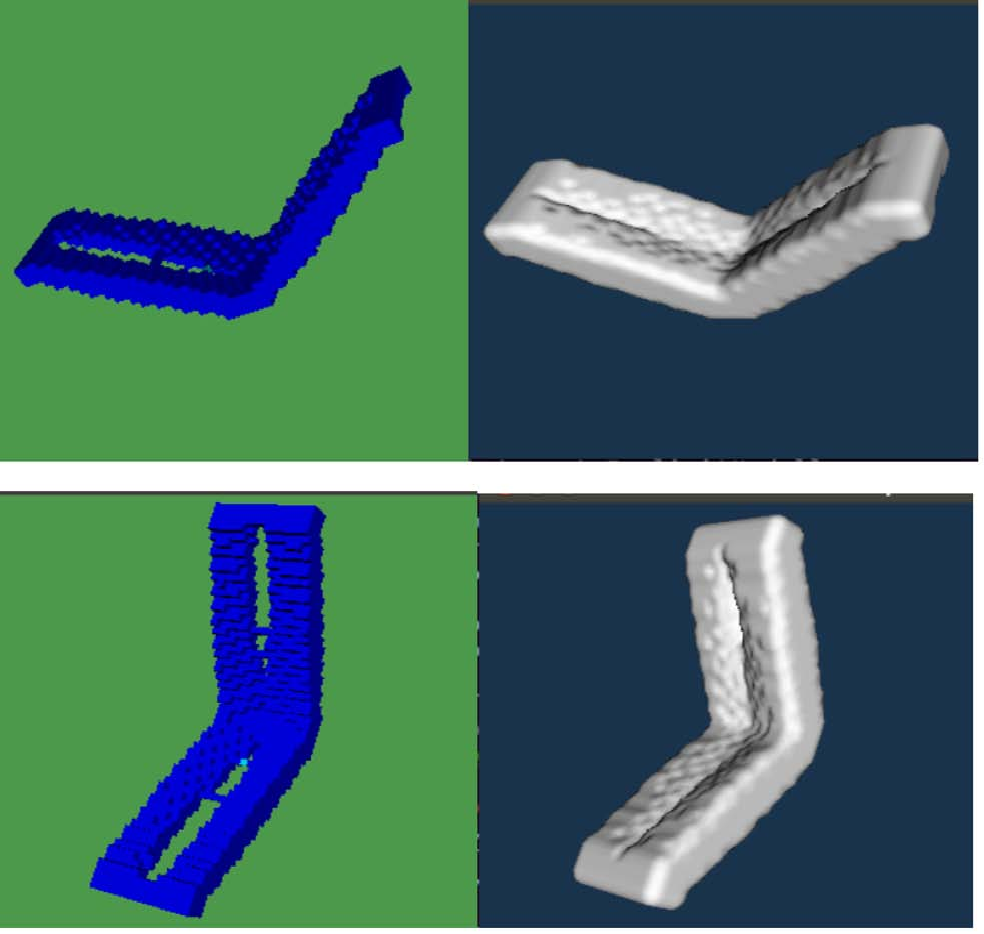
\includegraphics{Pictures/contouring.pdf}}\\
   \caption{Contour Filtering tool after Implicit Modelling. The original geometry (left) is an optimized geometry output from ToPy (see \autoref{sec:ToPy}. Note that some essential features of the geometry after the process (right) are lost, such as the holes through the structure.}
   \label{fig:contouring}
\end{figure}

% I don't understand this sentence - I'll leave it out for now.

%A further idea to solve this problem is to first convert the volume data into point data
%and only then present it to the \textit{Contour Filtering} tool .

In order to reduce computational costs of the following NURBS fitting process (see \autoref{sec:NURBS}) we also need to create a coarser mesh of polygons from the fine one. The number of triangles that represent the
isosurface can here be reduced with the VTK Decimation tool mentioned above. A smoothing step is however necessary in-between
to get the new connections right. As can be seen in \autoref{fig:Decimation}, a 50 \% reduction of the
triangles barely provides a noticeable difference, and even with a 90 \% reduction it is difficult to see a difference. Triangle meshes can be easily coarsened since there are many open source algorithms that reduce the number of triangles. %reference

\begin{figure}
\centering
   \scalebox{0.4}{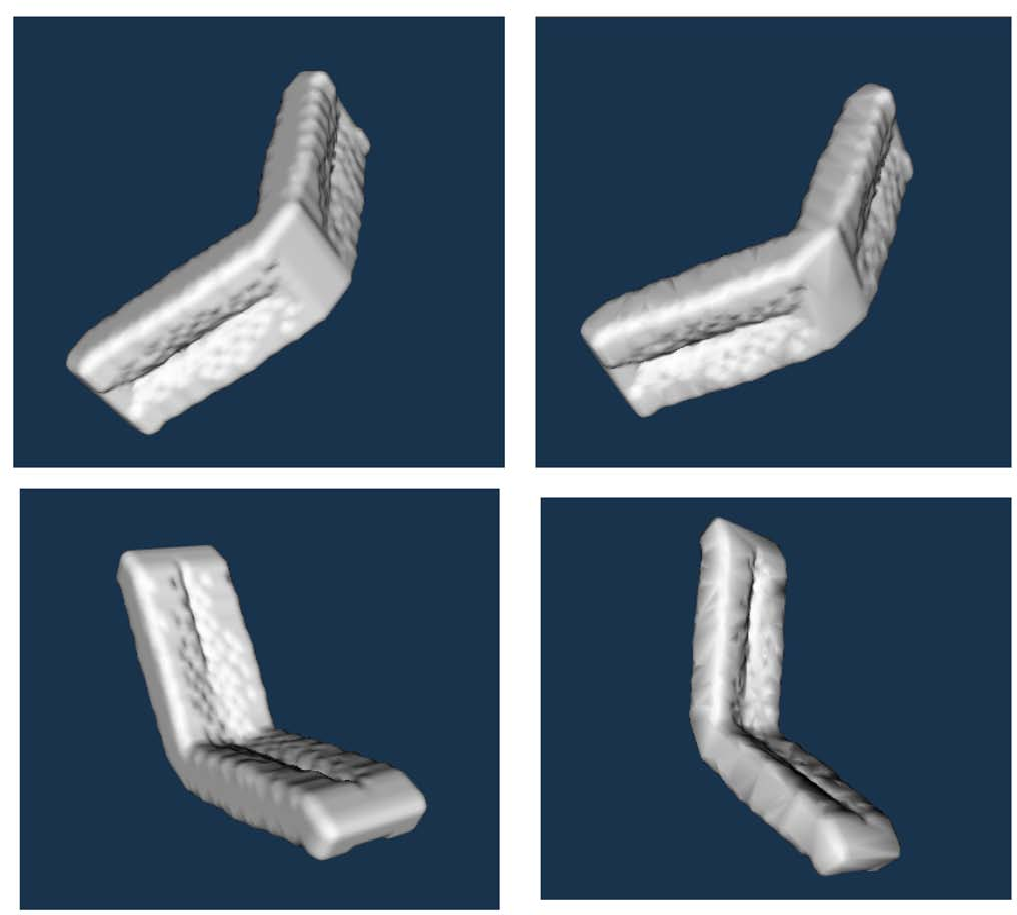
\includegraphics{Pictures/Decimation.pdf}}\\
   \caption{Decimation of triangles. \emph{Top:} 50\% reduction of triangle number from the object in \autoref{fig:contouring}. \emph{Lower:} 90\% reduction. The difference is barely noticable in both cases.}
   \label{fig:Decimation}
\end{figure}
\end{comment}
